%%%%%%%%%%%%%%%%%%%%%%%%%%%%%%%%%%%%%%%%%
% Programming/Coding Assignment
% LaTeX Template
%
% This template has been downloaded from:
% http://www.latextemplates.com
%
% Original author:
% Ted Pavlic (http://www.tedpavlic.com)
%
% Note:
% The \lipsum[#] commands throughout this template generate dummy text
% to fill the template out. These commands should all be removed when 
% writing assignment content.
%
% This template uses a Perl script as an example snippet of code, most other
% languages are also usable. Configure them in the "CODE INCLUSION 
% CONFIGURATION" section.
%
%%%%%%%%%%%%%%%%%%%%%%%%%%%%%%%%%%%%%%%%%

%----------------------------------------------------------------------------------------
%	PACKAGES AND OTHER DOCUMENT CONFIGURATIONS
%----------------------------------------------------------------------------------------

\documentclass{article}

\usepackage{fancyhdr} % Required for custom headers
\usepackage{lastpage} % Required to determine the last page for the footer
\usepackage{extramarks} % Required for headers and footers
\usepackage[usenames,dvipsnames]{color} % Required for custom colors
\usepackage{graphicx} % Required to insert images
\usepackage{subcaption}
\usepackage{listings} % Required for insertion of code
\usepackage{courier} % Required for the courier font
\usepackage{lipsum} % Used for inserting dummy 'Lorem ipsum' text into the template
\usepackage{amsmath} % Use for multiple line equations
% Margins
\topmargin=-0.45in
\evensidemargin=0in
\oddsidemargin=0in
\textwidth=6.5in
\textheight=9.0in
\headsep=0.25in

\linespread{1.1} % Line spacing

% Set up the header and footer
\pagestyle{fancy}
\lhead{\hmwkAuthorName} % Top left header
\chead{\hmwkClass\ (\hmwkClassTime): \hmwkTitle} % Top center head
%\rhead{\firstxmark} % Top right header
\lfoot{\lastxmark} % Bottom left footer
\cfoot{} % Bottom center footer
\rfoot{Page\ \thepage\ of\ \protect\pageref{LastPage}} % Bottom right footer
\renewcommand\headrulewidth{0.4pt} % Size of the header rule
\renewcommand\footrulewidth{0.4pt} % Size of the footer rule

\setlength\parindent{0pt} % Removes all indentation from paragraphs

%----------------------------------------------------------------------------------------
%	CODE INCLUSION CONFIGURATION
%----------------------------------------------------------------------------------------

\definecolor{MyDarkGreen}{rgb}{0.0,0.4,0.0} % This is the color used for comments
\lstloadlanguages{Perl} % Load Perl syntax for listings, for a list of other languages supported see: ftp://ftp.tex.ac.uk/tex-archive/macros/latex/contrib/listings/listings.pdf
\lstset{language=Perl, % Use Perl in this example
        frame=single, % Single frame around code
        basicstyle=\small\ttfamily, % Use small true type font
        keywordstyle=[1]\color{Blue}\bf, % Perl functions bold and blue
        keywordstyle=[2]\color{Purple}, % Perl function arguments purple
        keywordstyle=[3]\color{Blue}\underbar, % Custom functions underlined and blue
        identifierstyle=, % Nothing special about identifiers                                         
        commentstyle=\usefont{T1}{pcr}{m}{sl}\color{MyDarkGreen}\small, % Comments small dark green courier font
        stringstyle=\color{Purple}, % Strings are purple
        showstringspaces=false, % Don't put marks in string spaces
        tabsize=5, % 5 spaces per tab
        %
        % Put standard Perl functions not included in the default language here
        morekeywords={rand},
        %
        % Put Perl function parameters here
        morekeywords=[2]{on, off, interp},
        %
        % Put user defined functions here
        morekeywords=[3]{test},
       	%
        morecomment=[l][\color{Blue}]{...}, % Line continuation (...) like blue comment
        numbers=left, % Line numbers on left
        firstnumber=1, % Line numbers start with line 1
        numberstyle=\tiny\color{Blue}, % Line numbers are blue and small
        stepnumber=5 % Line numbers go in steps of 5
}

% Creates a new command to include a perl script, the first parameter is the filename of the script (without .pl), the second parameter is the caption
\newcommand{\perlscript}[2]{
\begin{itemize}
\item[]\lstinputlisting[caption=#2,label=#1]{#1.pl}
\end{itemize}
}

%----------------------------------------------------------------------------------------
%	DOCUMENT STRUCTURE COMMANDS
%	Skip this unless you know what you're doing
%----------------------------------------------------------------------------------------

% Header and footer for when a page split occurs within a problem environment
\newcommand{\enterProblemHeader}[1]{
%\nobreak\extramarks{#1}{#1 continued on next page\ldots}\nobreak
%\nobreak\extramarks{#1 (continued)}{#1 continued on next page\ldots}\nobreak
}

% Header and footer for when a page split occurs between problem environments
\newcommand{\exitProblemHeader}[1]{
%\nobreak\extramarks{#1 (continued)}{#1 continued on next page\ldots}\nobreak
%\nobreak\extramarks{#1}{}\nobreak
}

\setcounter{secnumdepth}{0} % Removes default section numbers
\newcounter{homeworkProblemCounter} % Creates a counter to keep track of the number of problems
\setcounter{homeworkProblemCounter}{-1}

\newcommand{\homeworkProblemName}{}
\newenvironment{homeworkProblem}[1][Part \arabic{homeworkProblemCounter}]{ % Makes a new environment called homeworkProblem which takes 1 argument (custom name) but the default is "Problem #"
\stepcounter{homeworkProblemCounter} % Increase counter for number of problems
\renewcommand{\homeworkProblemName}{#1} % Assign \homeworkProblemName the name of the problem
\section{\homeworkProblemName} % Make a section in the document with the custom problem count
\enterProblemHeader{\homeworkProblemName} % Header and footer within the environment
}{
\exitProblemHeader{\homeworkProblemName} % Header and footer after the environment
}

\newcommand{\problemAnswer}[1]{ % Defines the problem answer command with the content as the only argument
\noindent\framebox[\columnwidth][c]{\begin{minipage}{0.98\columnwidth}#1\end{minipage}} % Makes the box around the problem answer and puts the content inside
}

\newcommand{\homeworkSectionName}{}
\newenvironment{homeworkSection}[1]{ % New environment for sections within homework problems, takes 1 argument - the name of the section
\renewcommand{\homeworkSectionName}{#1} % Assign \homeworkSectionName to the name of the section from the environment argument
\subsection{\homeworkSectionName} % Make a subsection with the custom name of the subsection
\enterProblemHeader{\homeworkProblemName\ [\homeworkSectionName]} % Header and footer within the environment
}{
\enterProblemHeader{\homeworkProblemName} % Header and footer after the environment
}

%----------------------------------------------------------------------------------------
%	NAME AND CLASS SECTION
%----------------------------------------------------------------------------------------

\newcommand{\hmwkTitle}{Assignment\ \#3} % Assignment title
\newcommand{\hmwkDueDate}{Monday,\ Mar\ 19,\ 2018} % Due date
\newcommand{\hmwkClass}{CSC411} % Course/class
\newcommand{\hmwkClassTime}{L2501} % Class/lecture time
\newcommand{\hmwkAuthorName}{Kaiyang Chen, Weixin Liu} % Your name

%----------------------------------------------------------------------------------------
%	TITLE PAGE
%----------------------------------------------------------------------------------------

\title{
\vspace{2in}
\textmd{\textbf{\hmwkClass:\ \hmwkTitle}}\\
\normalsize\vspace{0.1in}\small{Due\ on\ \hmwkDueDate}\\
\vspace{0.1in}
\vspace{3in}
}

\author{\textbf{\hmwkAuthorName}}
%\date{} % Insert date here if you want it to appear below your name

%----------------------------------------------------------------------------------------

\begin{document}

\maketitle
\clearpage

%----------------------------------------------------------------------------------------
%	PROBLEM 0
%----------------------------------------------------------------------------------------

\begin{homeworkProblem}
This project works with a fake and real news data set avaiable on:
\\
\texttt{https://www.kaggle.com/mrisdal/fake-news/data}
\\and
\texttt{https://www.kaggle.com/therohk/million-headlines}
\\
Three models will be built in this project - Naive bayers, Logistic regression and Decision tree. For detail implementation of these methods, please review the python file.
\end{homeworkProblem}
\clearpage

%----------------------------------------------------------------------------------------
%	PROBLEM 1
%----------------------------------------------------------------------------------------

% To have just one problem per page, simply put a \clearpage after each problem

\begin{homeworkProblem}

\noindent \textit{Dataset description}
\\[10pt]
The datasets are text files whose each line represents one new title. First, we listed the top 10 most prevailing words in both fake news and real news and plot the i-th most prevailing word vs. its number of appearance in Figure~\ref{fig:part1}. Note that even one word is appeard multiple times in one headline, we only count it as appeared once.\\
\begin{lstlisting}
the 1-th most prevealing word in fake news is trump :1282
the 2-th most prevealing word in fake news is to :366
the 3-th most prevealing word in fake news is the :363
the 4-th most prevealing word in fake news is donald :228
the 5-th most prevealing word in fake news is in :218
the 6-th most prevealing word in fake news is of :197
the 7-th most prevealing word in fake news is for :196
the 8-th most prevealing word in fake news is a :172
the 9-th most prevealing word in fake news is and :166
the 10-th most prevealing word in fake news is on :160

the 1-th most prevealing word in real news is trump :1739
the 2-th most prevealing word in real news is donald :828
the 3-th most prevealing word in real news is to :380
the 4-th most prevealing word in real news is us :230
the 5-th most prevealing word in real news is trumps :219
the 6-th most prevealing word in real news is in :213
the 7-th most prevealing word in real news is on :204
the 8-th most prevealing word in real news is of :181
the 9-th most prevealing word in real news is says :178
the 10-th most prevealing word in real news is for :171
\end{lstlisting}

\begin{figure*}[!ht]
\centering
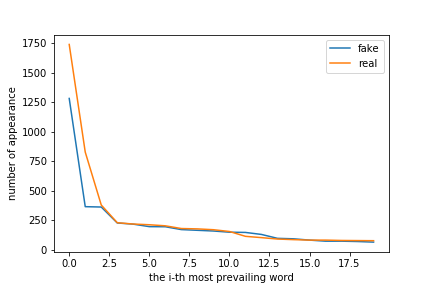
\includegraphics[scale = 0.7 ]{part1.png}
\caption{the i-th most prevailing word vs. its number of appearance}
\label{fig:part1}
\end{figure*}

From the results shown above, "trump" appears more than 1000 times in both fake and real news. Thus "trump" may not be very useful in predicting the news being real or fake. Besides that, most words only appear less than 250 times in both fake and real news. And about half of the top 10 words are stop-word.\\

In order to see if there exists such words that its appearance can distinguish real or fake news, we computed the difference of the number of appearance of each words in both cases, checked the most different words. We included some words that may be useful in classifying fake or real headlines below in Table ~\ref{table:part1}.

\begin{table}[!ht]
    \centering
    \begin{tabular}{ |c|c|c|c| } 
        \hline
        word & \# in fake news & \# in fake news & \# difference \\ 
        \hline
        korea & 0 & 79 & 79 \\ 
        \hline
        turnbull & 0 & 55 & 55 \\ 
        \hline
        north & 33 & 1 & 32 \\ 
        \hline
    \end{tabular}
    \caption{Count of words in real and fake headlines}
    \label{table:part1}
\end{table}

In general, there are many words that can help classifying real or fake news headlines, but there are also a lot stop-words and words such as "trump" that may lead to poor performance. If we can handle these words in our algorithm, then it is feasible to predict whether a headline is real or fake news.

The code used to split the data is pasted below:
\begin{lstlisting}
# Since we use np.random.seed() to randomize the data
# We convert our input into array
# But we use list manipulation later on, so we convet array back to list after shuffle
np.random.seed(0)
fakeDataCopy = copy.deepcopy(fakeData)
realDataCopy = copy.deepcopy(realData)
fakeDataArray = np.array(fakeDataCopy)
realDataArray = np.array(realDataCopy)
np.random.shuffle(fakeDataArray)
np.random.shuffle(realDataArray)

fakeTrain = fakeDataArray[:int(len(fakeDataArray)*0.7)]
fakeVali = fakeDataArray[int(len(fakeDataArray)*0.7):int(len(fakeDataArray)*0.85)]
fakeTest = fakeDataArray[int(len(fakeDataArray)*0.85):]

realTrain = realDataArray[:int(len(realDataArray)*0.7)]
realVali = realDataArray[int(len(realDataArray)*0.7):int(len(realDataArray)*0.85)]
realTest = realDataArray[int(len(realDataArray)*0.85):]

fakeTrain = fakeTrain.tolist()
fakeVali = fakeVali.tolist()
fakeTest = fakeTest.tolist()

realTrain = realTrain.tolist()
realVali = realVali.tolist()
realTest = realTest.tolist()
\end{lstlisting}

\end{homeworkProblem}
\clearpage
%----------------------------------------------------------------------------------------
%	PROBLEM 2
%----------------------------------------------------------------------------------------

\begin{homeworkProblem}
\noindent \textit{Implement Naive Bayes}
\\[10pt]
In order to tune the parameters of the prior: $m$ and $\hat{p}$, we tried different combination of $m$ and $\hat{p}$ and chose the combination with best performance on validation set. The range of $m$ we chose is \texttt{[10**exp for exp in np.arange(0,2.5,0.5, dtype=float)]} and the range of $\hat{p}$ is \texttt{[10**exp for exp in np.arange(-5,0, dtype=float)]}. In other words, we take $m = 10^0, 10^{0.5}, 10^1, ..., 10^{2}$ and $\hat{p} = 10^{-5}, 10^{-4}, ..., 10^{-1}$.
\\
When $m = 10^{0.5} = 3.1623, \hat{p} = 10^{-1} = 0.10000$, the performance on validation set is highest: 0.88571. The Figure~\ref{fig:part2} below is a contour plot of performance on validation set with difference choice of $m$ and $\hat{p}$.

\begin{figure*}[!ht]
\centering
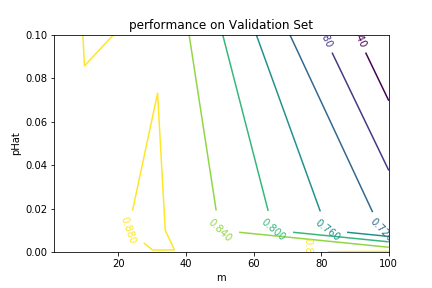
\includegraphics[scale = 0.7 ]{part2.png}
\caption{contour plot of performance on validation set with difference choice of $m$ and $\hat{p}$}
\label{fig:part2}
\end{figure*}

With m = 3.1623, pHat = 0.10000:\\
Performance on Training Set is 0.96193\\
Performance on Validation Set is 0.88776\\
Performance on Test Set is 0.84725\\

In perdiciton in Naive Bayes algorithm, 
\begin{align*}
    C & = argmax_{c}P(x_{1},...,x_{n}|c)P(c)\\
      & = P(x_{1}|c)P(x_{2}|c)...P(x_{n-1}|c)P(x_{n}|c)P(c)\\
      & = P(c)\prod_{i}{P(x_{i}|c)}
\end{align*}
$\prod_{i}{P(x_{i}|c)}$ involves multiplication of many small numbers, which may cause arithmetric underflow. There are only two classes (real / fake news). Therefore, we can predict class by comparing the log of the above expression to avoid arithmetic underflow. To be precise, we compare 
$$log(P(c)\prod_{i}{P(x_{i}|c))} = logP(c) + \sum_{i}logP(x_{i}|c)$$
Therefore, we can simply compare the value of the above expression for the two cases (two C's), we assign the hypothesis of real news headline if the $logP(c=real) + \sum_{i}logP(x_{i}|c=real)$ is geater than that of $c = false$, and vise versa. Thus we can compute the performance by comparing to the original label.
\\
The code for Naive Bayes prediction \texttt{NaiveBayes()} and prediciton \texttt{Performance()} used in this part is pasted below:
\\[5pt]
\begin{lstlisting}
def Performance(wordsProb, p_fake, fakeData, realData):
    '''
    input:
        wordsProb: a dictionary whose key is the word xi and value is a list: 
            the first element in sublist is P(xi=1|fake), 
            the second element is sublist is P(xi=1|real).
        
        fakeData: a list of lists of words, each sublist is a single news. 
        realData: a list of lists of words, each sublist is a single news. 
        p_fake: P(fake)
    output:
        percentage performance on fakeData and real Data

    Note that in here, when we are comparing whether a news is characterized as 
    fake or real based on this log of the probability (or numerator of the Naive Bayes law)
    because if we do not take logarithm, we will have underflow
    '''
    correct = 0.0
    for i in fakeData:
        fakeProb = 0.0
        realProb = 0.0
        for j in wordsProb:
            if j in i:
                fakeProb += math.log(wordsProb[j][0])
                realProb += math.log(wordsProb[j][1])
            else:
                fakeProb += math.log(1-wordsProb[j][0])
                realProb += math.log(1-wordsProb[j][1])
        fakeProb += math.log(p_fake)
        realProb += math.log(1-p_fake)
        
        if fakeProb >= realProb:
            correct += 1

    for i in realData:
        fakeProb = 0.0
        realProb = 0.0
        for j in wordsProb:
            if j in i:
                fakeProb += math.log(wordsProb[j][0])
                realProb += math.log(wordsProb[j][1])
            else:
                fakeProb += math.log(1-wordsProb[j][0])
                realProb += math.log(1-wordsProb[j][1])
        fakeProb += math.log(p_fake)
        realProb += math.log(1-p_fake)

        if fakeProb <= realProb:
            correct += 1        

    perf = float(correct)/float(len(fakeData)+len(realData))
    return perf
    
def NaiveBayes(m, pHat, ifprint = True, ifreturnProb = False):
    '''
    Given m and pHat, return the performance on Training set, 
    Validation set and Test set.
    '''
    if ifprint:
        print "running NaiveBayes with m = %05.5f, pHat = %05.5f"%(m, pHat)

    wordsProb={}  #a dictionary whose key is the word xi and value is a list: 
                  #the first element in sublist is P(xi=1|fake), 
                  #the second element is sublist is P(xi=1|real).
    for i in wordList:
        if i in fakeWordsCountsTrain:
            p_x_fake = float(fakeWordsCountsTrain[i] + m*pHat)/float(len(fakeTrain) + m)
        else:
            p_x_fake = float(m*pHat)/float(len(fakeTrain) + m)
        if i in realWordsCountsTrain:
            p_x_real = float(realWordsCountsTrain[i] + m*pHat)/float(len(realTrain) + m)
        else:
            p_x_real = float(m*pHat)/float(len(realTrain) + m)
        wordsProb[i] = [p_x_fake,p_x_real]

    p_fake = float(len(fakeTrain))/float(len(realTrain) + len(fakeTrain)) #P(fake)
    
    perfTrain = Performance(wordsProb, p_fake, fakeTrain, realTrain)
    perfVali = Performance(wordsProb, p_fake, fakeVali, realVali)
    perfTest = Performance(wordsProb, p_fake, fakeTest, realTest)
    
    if ifreturnProb:
        return perfTrain, perfVali, perfTest, wordsProb, p_fake
    else:
        return perfTrain, perfVali, perfTest
\end{lstlisting}
\end{homeworkProblem}
\clearpage



%----------------------------------------------------------------------------------------
%	PROBLEM 3
%----------------------------------------------------------------------------------------

\begin{homeworkProblem}
\noindent \textit{Specific words' effect on the prediction}
\\[10pt]
In this part, we use $m = 3.1623$ and $\hat{p} = 0.10000$, as they were proven to be the optimal chioce in Part 2
\\[10pt]
\noindent \textbf{\textit{Part 3a)}}
\\[10pt]
To find the top 10 words whose presence most strongly predicts the news is real / fake, we perform following action: We first calculate the probability of indicating a headline is real or fake, given the word presence, note that this probability is taken account of the prior (probability of real / fake headline) and normalized. Then, we take the difference between the probability of indicating fake and real headline. The greatest 10 (positive) differences corresponds to the 10 words whose presence most strongly predicts the news is fake. The 10 most negative differences corresponds to the 10 words whose presence most strongly predicts the news is real.
\\
To find the top 10 words whose absence most strongly predicts the news is real / fake, we perform similar situation as above. However, the probability of a word being absent is (1 - P(word being present)), we then multiply this to the prior and normalize the probability. After that, we can take the difference and find the top 10 words, just like demonstrated above.
\\
The results are:
\\
The top 10 words whose presence most strongly predicts that the news is real are: \\
"korea", "turnbull", "travel", "australia", "trade", "refugee", "tax", "debate", "paris", "defends"
\\
\begin{center}
    \begin{tabular}{|c|c|c|c|}
    \hline \textbf{word} &  \textbf{P(fake$\|$x=presence)} &  \textbf{P(real$\|$x=presence)} &  \textbf{Difference} \\ \hline
    korea & 0.0075868 & 0.9924132 & 0.9848263 \\ \hline
    turnbull & 0.0086224 & 0.9913776 & 0.9827552 \\ \hline
    travel & 0.0099853 & 0.9900147 & 0.9800294 \\ \hline
    australia & 0.0114308 & 0.9885692 & 0.9771384 \\ \hline
    trade & 0.0153090 & 0.9846910 & 0.9693820 \\ \hline
    refugee & 0.0160888 & 0.9839112 & 0.9678225 \\ \hline
    tax & 0.0169523 & 0.9830477 & 0.9660955 \\ \hline
    debate & 0.0169523 & 0.9830477 & 0.9660955 \\ \hline
    paris & 0.0169523 & 0.9830477 & 0.9660955 \\ \hline
    defends & 0.0202056 & 0.9797944 & 0.9595887 \\ \hline
    \end{tabular}
\end{center}
The top 10 words whose absence most strongly predicts that the news is real are: \\
"trump", "the", "to", "hillary", "a", "is", "for", "and", "clinton", "of"
\\
\begin{center}
    \begin{tabular}{|c|c|c|c|}
    \hline  \textbf{word} &  \textbf{P(fake$\|$x=absence)} &  \textbf{P(real$\|$x=absence)} &  \textbf{Difference} \\ \hline
    trump & 0.0734549 & 0.9265451 & 0.8530901 \\ \hline
    the & 0.3438503 & 0.6561497 & 0.3122995 \\ \hline
    to & 0.3712430 & 0.6287570 & 0.2575139 \\ \hline
    hillary & 0.3743025 & 0.6256975 & 0.2513950 \\ \hline
    a & 0.3748828 & 0.6251172 & 0.2502344 \\ \hline
    is & 0.3772314 & 0.6227686 & 0.2455372 \\ \hline
    for & 0.3786403 & 0.6213597 & 0.2427193 \\ \hline
    and & 0.3793777 & 0.6206223 & 0.2412445 \\ \hline
    clinton & 0.3830213 & 0.6169787 & 0.2339573 \\ \hline
    of & 0.3835959 & 0.6164041 & 0.2328082 \\ \hline
    \end{tabular}
\end{center}
The top 10 words whose presence most strongly predicts that the news is fake are: \\
"breaking", "3", "soros", "u", "daily", "woman", "steal", "reason", "endingfed", "these"
\\
\begin{center}
    \begin{tabular}{|c|c|c|c|}
    \hline  \textbf{word} &  \textbf{P(fake$\|$x=presence)} &  \textbf{P(real$\|$x=presence)} &  \textbf{Difference} \\ \hline
    breaking & 0.9809651 & 0.0190349 & 0.9619302 \\ \hline
    3 & 0.9783634 & 0.0216366 & 0.9567269 \\ \hline
    soros & 0.9767763 & 0.0232237 & 0.9535527 \\ \hline
    u & 0.9767763 & 0.0232237 & 0.9535527 \\ \hline
    daily & 0.9727836 & 0.0272164 & 0.9455671 \\ \hline
    woman & 0.9727836 & 0.0272164 & 0.9455671 \\ \hline
    steal & 0.9702239 & 0.0297761 & 0.9404478 \\ \hline
    reason & 0.9702239 & 0.0297761 & 0.9404478 \\ \hline
    endingfed & 0.9671328 & 0.0328672 & 0.9342656 \\ \hline
    these & 0.9671328 & 0.0328672 & 0.9342656 \\ \hline
    \end{tabular}
\end{center}
The top 10 words whose absence most strongly predicts that the news is fake are: \\
"donald", "trump", "us", "says", "ban", "north", "korea", "turnbull", "travel", "australia"
\\
\begin{center}
    \begin{tabular}{|c|c|c|c|}
    \hline  \textbf{word} &  \textbf{P(fake$\|$x=absence)} &  \textbf{P(real$\|$x=absence} &  \textbf{Difference} \\ \hline
    donald & 0.4874281 & 0.5125719 & 0.0251437 \\ \hline
    trumps & 0.4245949 & 0.5754051 & 0.1508102 \\ \hline
    us & 0.4197479 & 0.5802521 & 0.1605042 \\ \hline
    says & 0.4119073 & 0.5880927 & 0.1761853 \\ \hline
    ban & 0.4061333 & 0.5938667 & 0.1877335 \\ \hline
    north & 0.4050472 & 0.5949528 & 0.1899057 \\ \hline
    korea & 0.4045909 & 0.5954091 & 0.1908182 \\ \hline
    turnbull & 0.4036933 & 0.5963067 & 0.1926135 \\ \hline
    travel & 0.4027996 & 0.5972004 & 0.1944008 \\ \hline
    australia & 0.4020875 & 0.5979125 & 0.1958250 \\ \hline
    \end{tabular}
\end{center}

From above tables, it is clear that the presence of words has larger influence on predicting whether the headline is real or fake news. This is because the absolute difference between predicting a news is real/fake given the presence of the word (1st and 3rd table) is a lot larger than the absolute difference between predicting a news is real/fake given the absence of the word (2nd and 4th table). 
\\[5pt]

The code to perform above action is included below:
\begin{lstlisting}
perfTrain, perfVali, perfTest, wordsProb, p_fake = \
    NaiveBayes(3.1623, 0.10000, ifprint = False, ifreturnProb = True)
presenceFakeWordsProb = {}
presenceRealWordsProb = {}
absenceFakeWordsProb = {}
absenceRealWordsProb = {}
presenceWordsProbDiff = {}
absenceWordsProbDiff = {}
for i in wordsProb:
    p_presence_fake_p_fake = wordsProb[i][0]*p_fake
    p_presence_real_p_real = wordsProb[i][1]*(1-p_fake)
    presenceFakeWordsProb[i] = p_presence_fake_p_fake \
        /(p_presence_fake_p_fake+p_presence_real_p_real)
    presenceRealWordsProb[i] = p_presence_real_p_real \
        /(p_presence_fake_p_fake+p_presence_real_p_real)
    presenceWordsProbDiff[i] = presenceFakeWordsProb[i]-presenceRealWordsProb[i]
    
    p_absence_fake_p_fake = (1-wordsProb[i][0])*p_fake
    p_absence_real_p_real = (1-wordsProb[i][1])*(1-p_fake)
    absenceFakeWordsProb[i] = p_absence_fake_p_fake \
        /(p_absence_fake_p_fake+p_absence_real_p_real)
    absenceRealWordsProb[i] = p_absence_real_p_real \
        /(p_absence_fake_p_fake+p_absence_real_p_real)
    absenceWordsProbDiff[i] = absenceFakeWordsProb[i]-absenceRealWordsProb[i] 
    
presenceWordsProbDiffOrdered = sorted(presenceWordsProbDiff, \
    key = presenceWordsProbDiff.__getitem__, reverse=True)
absenceWordsProbDiffOrdered = sorted(absenceWordsProbDiff, \
    key = absenceWordsProbDiff.__getitem__, reverse=True)



for i in np.arange(-1,-11,-1):
    word = presenceWordsProbDiffOrdered[i]
    print "the %i-th strongly predicts real news with its presence is %s, \
        with P(fake|x=presence)=%05.5f, P(real|x=presence)=%05.5f" \
        %(-i,word,presenceFakeWordsProb[word],presenceRealWordsProb[word])
print "\n"
for i in np.arange(-1,-11,-1):
    word = absenceWordsProbDiffOrdered[i]
    print "the %i-th strongly predicts real news with its absence is %s, \
        with P(fake|x=absence)=%05.5f, P(real|x=absence)=%05.5f" \ 
        %(-i,word,absenceFakeWordsProb[word],absenceRealWordsProb[word])
print "\n"

for i in range(0,10):
    word = presenceWordsProbDiffOrdered[i]
    print "the %i-th strongly predicts fake news with its presence is %s, \
        wwith P(fake|x=presence)=%05.5f, P(real|x=presence)=%05.5f" \
        %(i+1,word,presenceFakeWordsProb[word],presenceRealWordsProb[word])
print "\n"  
for i in range(0,10):
    word = absenceWordsProbDiffOrdered[i]
    print "the %i-th strongly predicts fake news with its absence is %s, \
        with P(fake|x=absence)=%05.5f, P(real|x=absence)=%05.5f" \ 
        %(i+1,word,absenceFakeWordsProb[word],absenceRealWordsProb[word])
print "\n"
\end{lstlisting}


\end{homeworkProblem}
\clearpage

\noindent \textbf{\textit{Part 3b)}}
\\[10pt]
We use the result from Part 3a), find the top 10 words for each chactergory that are not "stopwords".
\\[5pt]
The results are the following:
\\
The 10 non-stopwords whose presence most strongly predict that the news is real are: \\
"korea", "turnbull", "travel", "australia", "trade", "refugee", "tax", "debate", "paris", "defends"
\\
The 10 non-stopwords whose absence most strongly predict that the news is real are: \\
"trump", "hillary", "clinton", "just", "obama", "new", "news", "america", "supporter", "campaign"
\\
The 10 non-stopwords whose presence most strongly predict that the news is fake are: \\
"breaking", "3", "soros", "u", "daily", "woman", "steal", "reason", "endingfed", "d"
\\
The 10 non-stopwords whose absence most strongly predict that the news is fake are: \\
"donald", "trump", "says", "ban", "north", "korea", "turnbull", "travel", "australia", "china"
\\

\noindent \textbf{\textit{Part 3c)}}
\\[10pt]
It makes sense to remove stop words because they do not usually add meaningful information to the headlines, from human perspective. Therefore it will not help the classification, intuitively.
On the other hand, it make sense to keep stop words because statistically, some of these words are significant in classifying real and fake news, especially in those words whose absence most strongly predicts that the news is real. They in fact helps the classification.

\clearpage



%----------------------------------------------------------------------------------------
%	PROBLEM 4
%----------------------------------------------------------------------------------------

\begin{homeworkProblem}
\noindent \textit{Logistic Regression}
\\[10pt]
\noindent \textit{Input, output, and parameter of the model}
\\[5pt]
The logistic regression takes an input matrix of size $m \times n$, where m is the number of all the distinct words that appear in all the headlines, and n is the number of total headlines (real + fake). The k-th element of $h$-th column vector ($h$-th headline) = 1 if $k$-th keyword appears in the headline $h$, and 0 otherwise. The label, Y, is a $1 \times n$, with each element = 1 if the news is fake, and = 0 if the news is real. The output of the logistic regression is a $1 \times n$ vector, each element representing the hypothesis of the logistic regression. 
\\
The cost function and parameter of the logistic regression is the following:
\begin{itemize}
    \item Cross-entropy is used as the cost function.
    \item Learning rate $\alpha = 0.005$
    \item Weights are initialized to a normal distribution with mean = 0 and standard deviation = 0.0001
    \item Maximum iteration is set to 3000.
    \item A L-2 regulazation term with $\lambda = 0.1$ is used. This choice is explained in detail below in this Part.
\end{itemize}

\noindent \textit{Performance}
\\[5pt]
The learning curve of the logistic regression model is shown below in Figure~\ref{fig:part4_learningCurve}.

\begin{figure*}[!ht]
\centering
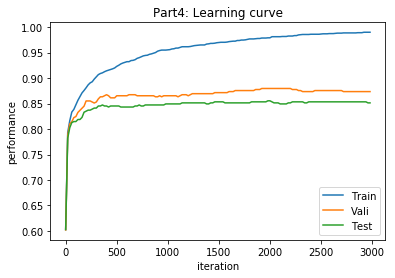
\includegraphics[scale = 0.7 ]{part4_learningCurve.png}
\caption{Learning curve of logistic regression}
\label{fig:part4_learningCurve}
\end{figure*}

The final performance of the model is following:
\begin{itemize}
    \item Training set accuracy 0.98371
    \item Validation set accuracy 0.8755
    \item Testing set accuracy 0.88540
\end{itemize}

\clearpage

\noindent \textit{Regularization parameter}
\\[5pt]
In this logistic regression model, we impose a L-2 regularization term. Specifically, the cross-entropy cost function is modified as follows:
$$Cost = -\sum_j(y_jlog(\theta^TX_j)+(1-y_j)log(1-\theta^TX_j)) + \lambda \Vert \theta^2 \Vert$$
In order to pick the most suitable $\lambda$, we try $\lambda = 10^{-3}, 10^{-2.5}, 10^{-2}, 10^{-1.5}, 10^{-0.5}, 10^{0}$ and plot the performance on Validation set with different $\lambda$. The plot is shown below in Figure~\ref{fig:part4_lambda}.

\begin{figure*}[!ht]
\centering
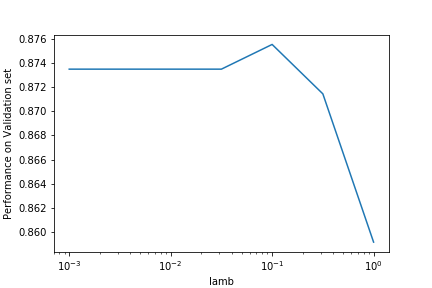
\includegraphics[scale = 0.7 ]{part4_lambda.png}
\caption{Performance on Validation Set with different $\lambda$s}
\label{fig:part4_lambda}
\end{figure*}

From the figure above, it is clear that with $\lambda = 10^{-1}$, we have the best performance on validation set, therefore $\lambda = 10^{-1}$ is chosen.

\end{homeworkProblem}
\clearpage




%----------------------------------------------------------------------------------------
%	PROBLEM 5
%----------------------------------------------------------------------------------------

\begin{homeworkProblem}
\noindent \textit{Logistic Regression and Naive Bayes Formulation}
\\[10pt]
\noindent \textit{Naive Bayers Formulation}
\\[5pt]
From lecture, it was shown/proven that the log odds of Naive Bayers can be represented as a logistic regression, assuming the Naive Bayers assumption holds. In this case, we have two cases: $c = 1$ represents the news is real, and $c = 0$ represents the news is fake.
\\
Then, the log odds of $y = c$ is, where y is our hypothesis of a headline is real or fake:
\\
\begin{align*}
log\frac{P(y=c|x_1,...,x_p)}{P(y=c'|x_1,...,x_p)} 
    &= log\frac{P(y=c)\Pi_jP(x_j|c)}{P(y=c')\Pi_jP(x_j|c')} \\
    & = log\frac{p(y=c)}{p(y=c')} + \Sigma_jlog\frac{P(x_j|y=c)}{P(x_j|y=c')} \\
    & = \beta_0 + \Sigma_j\beta_jx_j
\end{align*}
where 
$$\beta_0 = log\frac{P(y=c)}{P(y=c')} + \Sigma_jlog\frac{P(x_j = 0|y = c)}{P(x_j = 0|y = c')}$$
and
$$\beta_j = log\frac{P(x_j = 1|y = c)}{P(x_j = 1|y = c')}-log\frac{P(x_j = 0|y = c)}{P(x_j = 0|y = c')}$$
Note that $y=c$ represents one case, and $y=c'$ represents the other case. Since we only have two cases here, we can make the above formulation. $\beta_0$ is denoted as $\theta_0$ and $\beta_j$ is denoted as $\theta_j$ where $j = 1,2,...,k$ in the assignment handout.
\\[5pt]
Specifically, in this project (note all the count is referring to the number of (fake/real/total) news in the traning set), 
$$P(y = c) = \frac{count(fakeNews)}{count(total news)}$$
$$P(y = c') = \frac{count(realNews)}{count(total news)}$$
$$P(x_j=0|y=c) = 1-\frac{count(keyword_j;fakeNews) + m\hat{p}}{count(fakeNews)+m}$$
$$P(x_j=0|y=c') = 1-\frac{count(keyword_j;realNews) + m\hat{p}}{count(realNews)+m}$$
$$P(x_j=1|y=c) = \frac{count(keyword_j;fakeNews) + m\hat{p}}{count(fakeNews)+m}$$
$$P(x_j=1|y=c') = \frac{count(keyword_j;realNews) + m\hat{p}}{count(realNews)+m}$$
where $m$ and $\hat{p}$ are defined above in Part 2 and 3.
\\[5pt]
Now, looking at the Logistic regression formulatoin:
$$\theta_0 + \theta_{1}I_1(x) + \theta_{2}I_2(x) + ... + \theta_kI_k(x) > thr$$
the $\theta$'s are the $\beta$'s defined above, and the $I_1(x), I_2(x), ...I_k(x)$ are defined as the $x_j$ in the above formulation. Specifically, the $x$ is a $k \times 1$ column vector, with each element being $I_j(x), j = 1,..,k$. The $k$ represents total number of keywords appeared in all the headlines, and we use one-hot encoding to formulate $x$. This means that if $word_j$ is in this headline, then the j-th element of this headline (the $x$) will encodes to be 1. \\
For example, one possible $x$ can be:
$$x = \begin{bmatrix}
        0 \\
        0 \\
        \vdots \\
        1
        \\
        0 \\
        \vdots \\
        1\\
        \vdots \\
        0
        \end{bmatrix}$$
$I_j(x) = x_j(x) = 1$, if $word_j$ appears in the headline $x$; \\
$I_j(x) = x_j(x) = 0$, if $word_j$ not appear in the headline $x$.
\\[10pt]

\noindent \textit{Logistic Regression Formulation}
\\[5pt]
For logistic regression, the regression coefficient (weights) is a $k \times 1$ matrix, which directly corresponds to the $\theta$'s in the above formulation. The features also directly corresponds to the above one-hot key encoding of $x$, with each element being 1 if the word is in the headline, and 0 if not. 

\end{homeworkProblem}
\clearpage


%----------------------------------------------------------------------------------------
%	PROBLEM 6
%----------------------------------------------------------------------------------------

\begin{homeworkProblem}
\noindent \textit{Comparison between Naive Bayers and Logistic Regression}
\\[10pt]
\noindent \textbf{\textit{Part 6a)}}
\\[5pt]
The top 10 positive $\theta$'s and their corresponding words are listed below:

\begin{table}[!ht]
\centering
\begin{tabular}{|c|c|}
\hline
\textbf{Theta Value} & \textbf{Word} \\ \hline
2.3213573            & breaking      \\ \hline
2.2626210            & victory       \\ \hline
1.9604588            & hillary       \\ \hline
1.9514560            & support       \\ \hline
1.8439966            & are           \\ \hline
1.7549683            & watch         \\ \hline
1.7270442            & black         \\ \hline
1.6830737            & daily         \\ \hline
1.6427152            & 3             \\ \hline
1.6174283            & go            \\ \hline
\end{tabular}
\end{table}

The top 10 negative $\theta$'s and their corresponding words are listed below:

\begin{table}[!ht]
\centering
\begin{tabular}{|c|c|}
\hline
\textbf{Theta Value} & \textbf{Word} \\ \hline
-3.0053665           & trumps        \\ \hline
-2.0746956           & crawl         \\ \hline
-1.9956767           & us            \\ \hline
-1.9355898           & turnbull      \\ \hline
-1.9247129           & australia     \\ \hline
-1.7264927           & debate        \\ \hline
-1.6991252           & north         \\ \hline
-1.6660885           & tax           \\ \hline
-1.5726381           & trade         \\ \hline
-1.5100357           & donald        \\ \hline
\end{tabular}
\end{table}

Compare these list with those in part 3(a), we observe the following:
\begin{enumerate}
    \item There are some overlap between the words corresponding to the top 10 positive thetas and top 10 words whose presence most strongly predicts that the news is fake.
    \item There are some overlap between the words corresponding to the top 10 negative thetas and top 10 words whose presence most strongly predicts that the news is real.
\end{enumerate}
There are some overlap of words because the most positive theta indicates the presence of the word will tend to make the hypothesis value large. We defined as if the hypothesis value $>$ 0.5, then it is categorized as fake news. On the other hand, the most negative theta indicates the presence of the word will make the hypothesis value small by going into negative. We defined as if the hypothesis value is $<$ 0.5, then it is categorized as real news.
\\
But the lists of the words are not identical because of the Naive Bayers assumption. Under the ideal environment, where the keywords in the headlines are conditionally independent, Naive Bayers and logistic regression should produce the same result because they are essentially the same model. However, since we observe the results are different, it suggests that the Naive Bayers assumption may not hold perfectly here. It make sense because these headline words are collected from sentences, and their should be correlation between the words to some degree. 
\\[10pt]

\noindent \textbf{\textit{Part 6b)}}
\\[5pt]
The top 10 positive $\theta$'s and their corresponding words, ignoring all stop words, are listed below:

\begin{table}[!ht]
\centering
\begin{tabular}{|c|c|}
\hline
\textbf{Theta Value} & \textbf{Word} \\ \hline
2.3213573            & breaking      \\ \hline
2.2626210            & victory       \\ \hline
1.9604588            & hillary       \\ \hline
1.9514560            & support       \\ \hline
1.7549683            & watch         \\ \hline
1.7270442            & black         \\ \hline
1.6830737            & daily         \\ \hline
1.6427152            & 3             \\ \hline
1.5929630            & won           \\ \hline
1.5067344            & just          \\ \hline
\end{tabular}
\end{table}

The top 10 negative $\theta$'s and their corresponding words, ignoring all stop words, are listed below:

\begin{table}[!ht]
\centering
\begin{tabular}{|c|c|}
\hline
\textbf{Theta Value} & \textbf{Word} \\ \hline
-3.0053665           & trumps        \\ \hline
-2.0746956           & crawl         \\ \hline
-1.9355898           & turnbull      \\ \hline
-1.9247129           & australia     \\ \hline
-1.7264927           & debate        \\ \hline
-1.6991252           & north         \\ \hline
-1.6660885           & tax           \\ \hline
-1.5726381           & trade         \\ \hline
-1.5100357           & donald        \\ \hline
-1.4996588           & business      \\ \hline
\end{tabular}
\end{table}

Compare these list with those in part 3(b), we observe the following:
\begin{enumerate}
    \item When ignoring the stop words, there are some overlap between the words corresponding to the top 10 positive thetas and top 10 words whose presence most strongly predicts that the news is fake.
    \item When ignoring the stop words, there are some overlap between the words corresponding to the top 10 negative thetas and top 10 words whose presence most strongly predicts that the news is real.
\end{enumerate}
Note that this observation is similar to that in Part 6a), with the same underlying reason of the observation. 

\clearpage

\noindent \textbf{\textit{Part 6c)}}
\\[5pt]
In general, it is not a bad idea to use magnitude of the logistic regression parameters to indicate importance of a feature when the input is "normalized". If the features are not normalized, then features with smaller magnitude tends to have a larger regression parameter. Then, a larger regression parameter does not necessary corresponds to the importance of a feature, but just the "relative magnitude" of the feature.
\\
However, in our case, it is reasonable to use the magnitude because our input is either 1 or 0 to represent whether the word is present in the news headline.

\end{homeworkProblem}
\clearpage




%----------------------------------------------------------------------------------------
%	PROBLEM 7
%----------------------------------------------------------------------------------------

\begin{homeworkProblem}
\noindent \textit{Decision Tree Implementation}
\\[5pt]
In this section, a decision tree classifier to classify an email is fake or real is presented. The decision tree classifier is based on the package \texttt{sklean.tree}.
\\[5pt]
\noindent \textbf{\textit{Part 7a)}}
\\[5pt]
The training set input for the decision tree is a $n \times k$ matrix, where $n$ is number of the headlines in the training set, and $k$ is the number of total key words in all the headlines. We also use one-hot key encoding in this input. Note that this input is essentially the transpose of the input in logistic regression in Part 4, but without the bias term. The label for the input is a $n \times 1$ column matrix, with label 1 if the true label for the news is fake, and 0 if the true label for the news is real. Note that this is essentially the transpose of the label in logistic regression in Part 4. The validation and test set follow similar formation.
\\
Then, we use \texttt{sklean.tree} to train and evaluate the performance of the decision tree model. The only parameter that is tuned is the \texttt{max\_depth}. We use "entropy" for the criterion and default for all other parameters becasue "entropy" aligns with what we leanrt in this course. We tried \texttt{max\_depth} with value \texttt{[5, 10, 20, 30, 40, 50, 60, 70, 90, 110, 130, 160, 200, 250, 300, 350, 400]}. And the learning curve of performance vs. Max\_depth is plotted below in Figure~\ref{fig:part7_learningCurve}. Note that we choose a wide range of numbers with different frequency to spot possible overfit in the model.
\\
We choose the best performing max\_dept to be $70$. Because the performance keeps increasing before the max\_dept reaches $70$. And it is only when max\_dept = $400$, we have a 0.2\% better validation performance. We believe that at max\_dept = $70$, it is saver to say that the model has less overfitting, compared to larger max\_dept. The fact that the validation performance becomes worse after max\_dept = $70$ indicates a potential overfitting problem. Also, at this depth, the performance of the decision tree is decent.
\\
At max\_depth = $70$, we have:
\begin{itemize}
    \item accuracy on training set = 0.977242888403
    \item accuracy on validation set = 0.785714285714
    \item accuracy on test set = 0.747454175153
\end{itemize}


\begin{figure*}[!ht]
\centering
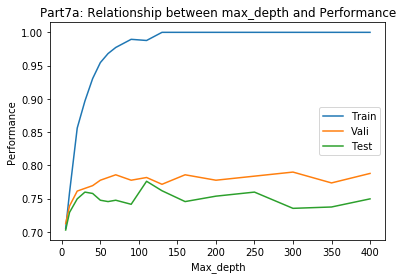
\includegraphics[scale = 0.7 ]{part7_learningCurve.png}
\caption{Performance of the decision tree with different maximum depths}
\label{fig:part7_learningCurve}
\end{figure*}

\clearpage

\noindent \textbf{\textit{Part 7b)}}
\\[5pt]
The visualization of the first two layers of the decision tree is included in Figure~\ref{fig:part7b} below.

\begin{figure*}[!ht]
\centering
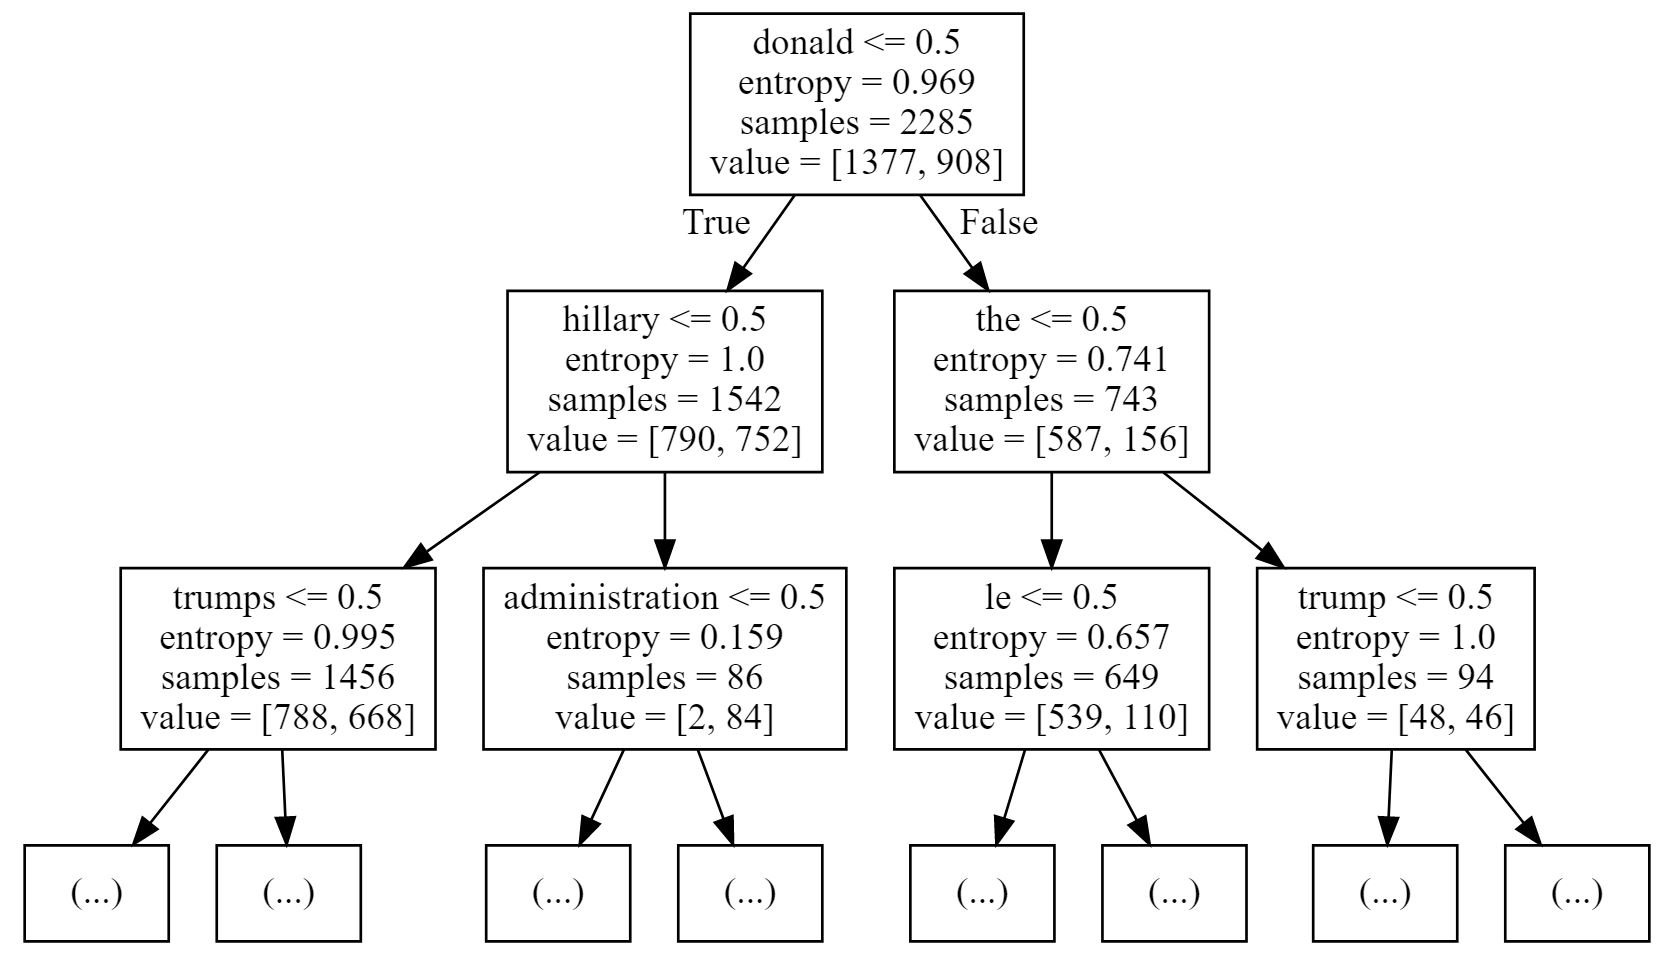
\includegraphics[scale = 0.7]{part7b.JPG}
\caption{Visualization of the first two layers of the tree}
\label{fig:part7b}
\end{figure*}

Some of the top keywords in decision tree also appears as the most important features in Naive Bayes(in Part 3a) and Logistic Regression(in Part 6a): "donald", "hillary", "trumps", "trump", "the" appear as the most important features both in decision tree and Naive Bayes; "donald", "hillary", "trumps" appear as the most important features both in decision tree and Logistic Regression. 

\noindent \textbf{\textit{Part 7c)}}
\\[5pt]
The performance of three classifiers on training, validation and test sets are summarized below in Table~\ref{table:part7}:

\begin{table}[!ht]
\centering
\caption{Performance of three classifiers}
\label{table:part7}
\begin{tabular}{|c|c|c|c|}
\hline
                             & \textbf{Naive Bayers} & \textbf{Logistic Regression} & \textbf{Decision Tree} \\ \hline
\textbf{Training Accuracy}   & 0.96193               & 0.98371                      & 0.97724                \\ \hline
\textbf{Validation Accuracy} & 0.88776               & 0.87551                      & 0.78571                \\ \hline
\textbf{Test Accuracy}       & 0.84725               & 0.85540                      & 0.74745                 \\ \hline
\end{tabular}
\end{table}



From above table, we can see that:
\begin{itemize}
    \item On training set, logistic regression performs the best, Naive Bayers performs the worst, but the all the accuracy are very high.
    \item On validation set, Naive Bayers performs the best, Decision Tree performs the worst. Note that the performance of Naive Bayers and logistic regression are similar and are significantly ($~10\%$) better than Decision tree.
    \item On test set, logistic regression performs the best. ecision Tree performs the worst. Note that the performance of Naive Bayers and logistic regression are similar and are significantly ($~10\%$) better than Decision tree.
    \item Therefore, we can conclude that Naive Bayers and logistic regression perform equally well; their performances are only differed by a small percentage. On the other hand, Decision Tree model has the worst performance in these three models. The fact that it has a much lower classification accuracy on the validation and test set indicates that it may be the model that overfit the most.
\end{itemize}

\end{homeworkProblem}
\clearpage

%----------------------------------------------------------------------------------------
%	PROBLEM 8
%----------------------------------------------------------------------------------------
\begin{homeworkProblem}
\noindent \textit{Mutual Information in Decision Tree}\\

The keyword chosen in the first split is "donald".
\begin{align*}
    I(Y,donald) &= H(Y) - H(Y\|donald)\\\\
    H(Y) &= -\frac{\#fake}{\#total}log_{2}\frac{\#fake}{\#total}-\frac{\#real}{\#total}log_{2}\frac{\#real}{\#total}\\
    &= -\frac{908}{1377+908}log_{2}\frac{908}{1377+908}-\frac{1377}{1377+908}log_{2}\frac{1377}{1377+908}=0.9693938491
\end{align*}
\begin{align*}
    H(Y\|donald) &= H(Y\|donald = 0)P(donald = 0) + H(Y\|donald = 1)P(donald = 1)\\
    &=(-\frac{\#fake\|donald = 0}{\#total\|donald = 0}log_{2}\frac{\#fake\|donald = 0}{\#total\|donald = 0}-\frac{\#real\|donald = 0}{\#total\|donald = 0}log_{2}\frac{\#real\|donald = 0}{\#total\|donald = 0})P(donald=0)\\
    &+(-\frac{\#fake\|donald = 1}{\#total\|donald = 1}log_{2}\frac{\#fake\|donald = 1}{\#total\|donald = 1}-\frac{\#real\|donald = 1}{\#total\|donald = 1}log_{2}\frac{\#real\|donald = 1}{\#total\|donald = 1})P(donald=0)\\
    &=(-\frac{752}{790+752}log_{2}\frac{752}{790+752}-\frac{790}{790+752}log_{2}\frac{790}{790+752})(\frac{790+752}{1377+908})\\
    &+(-\frac{156}{587+156}log_{2}\frac{156}{587+156}-\frac{587}{587+156}log_{2}\frac{587}{587+156})(\frac{587+156}{1377+908})\\
    &=0.6745402313+0.2410784799=0.9156187112\\\\
    I(Y,donald) &= H(Y) - H(Y\|donald) = 0.9693938491-0.9156187112 = 0.05377513794
\end{align*}

We also wrote a code for computing mutual information:
\begin{lstlisting}
def Entropy(num1, num2):
    '''
    input: num1 is the number of fake news given a condition
           num2 is the number of real news given a condition
    output: Entropy in this condition
    '''
    temp1 = float(num1)/float(num1+num2)
    temp2 = float(num2)/float(num1+num2)
    return -(temp1*math.log(temp1,2)+temp2*math.log(temp2,2))

def part8(word):
    '''
    input: xi
    output: I(Y,xi)
    '''
    H_Y = Entropy(len(fakeTrain),len(realTrain))
    
    numFakePresence = 0.0
    numRealPresence = 0.0
    numFakeAbsence = 0.0
    numRealAbsence = 0.0
    for i in fakeTrain:
        if word in i:
            numFakePresence += 1
        else:
            numFakeAbsence += 1
    for i in realTrain:
        if word in i:
            numRealPresence += 1
        else:
            numRealAbsence += 1
            
    H_Y_word = Entropy(numFakeAbsence, numRealAbsence)*((numFakeAbsence+numRealAbsence)\
    /(len(fakeTrain)+len(realTrain)))\
    +Entropy(numFakePresence,numRealPresence)*((numFakePresence+numRealPresence)\
    /(len(fakeTrain)+len(realTrain)))
    
    return H_Y - H_Y_word
\end{lstlisting}



\noindent \textbf{\textit{Part 8b)}}\\
The keyword that I chose is "hillary", and compute the mutual information is 0.029884513444737082 by calling $part8("hillary")$ (Note: $part8()$ is pasted above).\\
The value should be smaller than the value obtained in part8a, because the decision tree algorithm chooses keyword "donald" because it has the highest mutual information. If any word's mutual information is higher than that of "donald", the algorithm would have chosen the word with highest mutual information instead of "donald".



\end{homeworkProblem}
\clearpage
%----------------------------------------------------------------------------------------

\end{document}